% -----------------------------------------------
% Template for SMAC SMC 2013
% adapted and corrected from the template for SMC 2012, which was adapted from that of SMC 2011
% further updated for TENOR 2015, 2016 and 2017
% -----------------------------------------------

\documentclass{article}
\usepackage{tenor2017}
\usepackage{ifpdf}
\usepackage[english]{babel}
\usepackage{balance}
\usepackage{courier}

%%%%%%%%%%%%%%%%%%%%%%%% Some useful packages %%%%%%%%%%%%%%%%%%%%%%%%%%%%%%%
%%%%%%%%%%%%%%%%%%%%%%%% See related documentation %%%%%%%%%%%%%%%%%%%%%%%%%%
%\usepackage{amsmath} % popular packages from Am. Math. Soc. Please use the 
%\usepackage{amssymb} % related math environments (split, subequation, cases,
%\usepackage{amsfonts}% multline, etc.)
%\usepackage{bm}      % Bold Math package, defines the command \bf{}
%\usepackage{paralist}% extended list environments
%%subfig.sty is the modern replacement for subfigure.sty. However, subfig.sty 
%%requires and automatically loads caption.sty which overrides class handling 
%%of captions. To prevent this problem, preload caption.sty with caption=false 
%\usepackage[caption=false]{caption}
%\usepackage[font=footnotesize]{subfig}


%user defined variables
\def\papertitle{A Hierarchic Diff Algorithm for Collaborative Music Document Editing}
\def\firstauthor{Christopher Antila}
\def\secondauthor{Jeffrey Trevi\~{n}o}
\def\thirdauthor{Gabriel Weaver}

% adds the automatic
% Saves a lot of ouptut space in PDF... after conversion with the distiller
% Delete if you cannot get PS fonts working on your system.

% pdf-tex settings: detect automatically if run by latex or pdflatex
\newif\ifpdf
\ifx\pdfoutput\relax
\else
   \ifcase\pdfoutput
      \pdffalse
   \else
      \pdftrue
\fi

\ifpdf % compiling with pdflatex
  \usepackage[pdftex,
    pdftitle={\papertitle},
    pdfauthor={\firstauthor, \secondauthor, \thirdauthor},
    bookmarksnumbered, % use section numbers with bookmarks
    pdfstartview=XYZ % start with zoom=100% instead of full screen; 
                     % especially useful if working with a big screen :-)
   ]{hyperref}
  %\pdfcompresslevel=9

  \usepackage[pdftex]{graphicx}
  % declare the path(s) where your graphic files are and their extensions so 
  %you won't have to specify these with every instance of \includegraphics
  \graphicspath{{./figures/}}
  \DeclareGraphicsExtensions{.pdf,.jpeg,.png}

  \usepackage[figure,table]{hypcap}

\else % compiling with latex
  \usepackage[dvips,
    bookmarksnumbered, % use section numbers with bookmarks
    pdfstartview=XYZ % start with zoom=100% instead of full screen
  ]{hyperref}  % hyperrefs are active in the pdf file after conversion

  \usepackage[dvips]{epsfig,graphicx}
  % declare the path(s) where your graphic files are and their extensions so 
  %you won't have to specify these with every instance of \includegraphics
  \graphicspath{{./figures/}}
  \DeclareGraphicsExtensions{.eps}

  \usepackage[figure,table]{hypcap}
\fi

%setup the hyperref package - make the links black without a surrounding frame
\hypersetup{
    colorlinks,%
    citecolor=black,%
    filecolor=black,%
    linkcolor=black,%
    urlcolor=black
}


% Title.
% ------
\title{\papertitle}

% Authors
% Please note that submissions are NOT anonymous, therefore 
% authors' names have to be VISIBLE in your manuscript. 
%
% Single address
% To use with only one author or several with the same address
% ---------------
%\oneauthor
%   {\firstauthor} {Affiliation1 \\ %
%     {\tt \href{mailto:author1@adomain.org}{author1@adomain.org}}}

%Two addresses
%--------------
% \twoauthors
%   {\firstauthor} {Affiliation1 \\ %
%     {\tt \href{mailto:author1@adomain.org}{author1@adomain.org}}}
%   {\secondauthor} {Affiliation2 \\ %
%     {\tt \href{mailto:author2@adomain.org}{author2@adomain.org}}}

% Three addresses
% --------------
 \threeauthors
   {\firstauthor} {nCoda \\ %
     {\tt \href{mailto:christopher@antila.ca}{christopher@antila.ca}}}
   {\secondauthor} {California State University, Monterey Bay \\ %
     {\tt \href{mailto:jtrevino@csumb.edu}{jtrevino@csumb.edu}}}
   {\thirdauthor} { University of Illinois, Urbana-Champaign \\ %
     {\tt \href{mailto:gweaver@illinois.edu}{gweaver@illinois.edu}}}


% ***************************************** the document starts here ***************
\begin{document}
%
\capstartfalse
\maketitle
\capstarttrue
%
\begin{abstract}
We describe an application of hierarchic diff to the collaborative editing of tree-based music representations, using Zhang and Shasha's tree edit distance
algorithm, as implemented within the XUDiff tool: the edit distance between two trees is the minimum number of edit operations necessary
to transform one tree into another.  We consider common operations on the score tree -- deleting, changing, and appending tree nodes -- to derive a minimal edit sequence, known as an edit script, and we benchmark the widely used Longest Common Substring algorithm against our approach to demonstrate its superior performance.
\end{abstract}
%

\section{Introduction}\label{sec:introduction}
\subsection{The Least Common Subsequence Algorithm as Default Diff}
Traditional document comparison algorithms, such as the Unix diff,
takes two sequences of characters as input and outputs an edit script
to transform one sequence into another.  An edit script consists of a
sequence of edit operations (usually insert, delete, and update) to
modify transform the first sequence relative to some type of entity
such as characters, words, or lines.  The edit distance is the minimum
cost edit script given costs for each operation.  Typical algorithms
to compute the script and the cost are variants of the Least Common
Subsequence algorithm.  


This approach to document comparison works well in situations where
the inputs are sequences of characters and one wants to be
able to compare those sequences relative to characters, words, or
lines.  Unfortunately, however, many modern file formats rely on
hierarchical object models to encode multiple levels of meaning
(e.g. XML, blocks of code).  As such, different algorithms for
hierarchical structures become necessary.  

Consider the following two
problems that result from this mismatch between traditional diff tools
and their input.  First, comparing documents in terms of low-level
documents (e.g. lines) may not result in changes that are meaningful
to the domain since lines are often an artifact of presentation.  For
example, one can generate 'noisy diffs' by just changing whitespace.
Second, the manner in which one define document similarity may change
depending upon the task at hand.  A poet may get along fine comparing
texts in terms of lines, which reflect part of the structure of the
text.  A musician, however, may want to compare documents in terms of
additional information that is lost from a purely line-based
approach.  A similar demand is seen within other communities; scholars
may want to analyze and compare texts relative to other structures
such as paragraphs or sections.

% How do these problems specifically impact musicians?
\subsection{Collaborative Music Information Requires a Hierarchic Diff}
As alluded to above, these problems are of specific importance to
those in music, both in terms of usability as well as how one may want
to define 'meaning' and 'similarity' among musical documents.  First,
the 'noisy diff' problem, in reporting differences that are not
relevant to musicians creates a usability problem.  Although
programmers have become accustomed to noisy diffs and the work-arounds
they require, the low adoption rate of computer-driven music analytic
tools, and the general lack of comfort among music scholars with these
tools, suggest that a program producing diffs of meaningless changes
would be poorly received by the community.  Second, the meaning of
textually-encoded music always requires additional interpretation.
Therefore, a one-dimensional sequence of characters (the data
structure for which traditional diff was designed) will not allow
musicians to compare two interpretations of music.  

Instead, musicians
need the ability to compare music and its interpretation which may be
expressed hierarchically.  Therefore, musicians need the ability to
compare two versions of hierarchical structures.  Finally, musicians
may want to compare two versions of a composition, at different levels
of abstraction as represented by these hierarchical structures or
restrict comparison to entities with certain properties.  For example,
a musician may want to compare two versions of a composition in terms
of pitch class alone, or of higher-level features like phrase structure. Moreover, a musician may want to filter a composition to
compare the portions intended for a given musician or instrument type.

\section{Applying The Zhang and Shasha Algorithm}
\subsection{The Zhang and Shasha Algorithm}
Our initial approach uses Zhang and Shasha's tree edit distance
algorithm as implemented within the XUDiff tool \cite{Weaver:2013sl}.  The edit distance
between two trees is the minimum number of edit operations necessary
to transform one tree to another; the edit operations that we
consider consist of deleting, changing, and appending tree nodes. As
before, a sequence of edit operations between two trees is called an
edit script.

Our proposed approach leverages previous work from other domains both in
industry and in academia.  Within industry, there are proprietary
difference engines, such as the SmartDifferencer by Semantic Designs,
to compare source code in a variety of edit operations \cite{Designs:qm}.  Within
academia, the tree diffing problem has been long studied by
theoretical computer science \cite{Bille:2005ec}.  Different algorithms such as
subtree hashing and even using IDs to align subtrees before computing
similarity have been studied by researchers such as Chawathe et
al. and Cobena et al. \cite{Chawathe:1996jb,Cobena:2002gd}.  We employ the Zhang and Shasha tree
difference algorithm to solve the edit distance between trees \cite{Zhang:1989ec,Zhang:1989il}.

One benefit of this approach is that practitioners can choose a preferred level of abstraction (as defined by level within the tree) with
which to summarize a change and define 'similarity'.  As such, we
hypothesize that XUDiff, when applied to interpretations of music as
hierarchically encoded by the MEI object model, will be able to
address the problems mentioned above: comparing compositions in terms
of their meaning as expressed via a hierarchical interpretation of the
text and thereby reducing noisy comparisons.

%Figure ___ compares the two approaches.  THERE MAY BE A
%NICE USE FOR A DIAGRAM SIMILAR TO PAGE 51 IN MY THESIS.
 

\subsection{A Comparative Example}
Consider the case of a simple edit: the exchange of a staff's two voices -- that is, the upward-facing stems of voice one become the downward-facing stems of voice one, and vice versa (see figure 1). 


\begin{figure}[!htb]
\centering
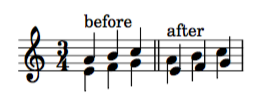
\includegraphics[width=0.8\columnwidth]{layers.png}
\caption{The figure above illustrates an edit that swaps the first and second voices in a staff. In common western notation, only stem direction reflects the change.}
\label{fig:example}
\end{figure}

While common western notation displays only a change of stem direction, a tree-based, hierarchic representation of this musical information must alter both the labeling and succession of elements: for example, in the widely used MEI XML representation of a music document, this initial representation,

\break

\begin{verbatim}
<staff n="1"> 
    <layer n="1">
        <note pname="a"/>
        <note pname="b"/>
        <note pname="c"/>
    </layer>
    <layer n="2">
        <note pname="e"/>
        <note pname="f"/>
        <note pname="g"/>
    </layer>
</staff>
\end{verbatim}

\noindent becomes, after the edit described,

\begin{verbatim}
<staff n="1">
    <layer n="1">
        <note pname="e"/>
        <note pname="f"/>
        <note pname="g"/>
    </layer>
    <layer n="2">
        <note pname="a"/>
        <note pname="b"/>
        <note pname="c"/>
    </layer>
</staff>
\end{verbatim}

\subsection{Benchmarking LCM against Zhang and Shasha}
How should a diff algorithm represent the described edit? The LCM algorithm yields a substantially different result from the Zhang and Shasha Algorithm. The Least Common Subsequence algorithm's line-based comparison yields a hierarchy-unaware diff with an edit distance of 10, half of which can be attributed to "noise" caused by the deletion of the layer element tags (see Figure 1). The Zhang and Shasha algorithm, on the other hand, reports an edit distance of 6 (3 for each layer) and can aggregate costs across the MEI hierarchy (see Figure 2).

\begin{figure*}[!htb]
\centering
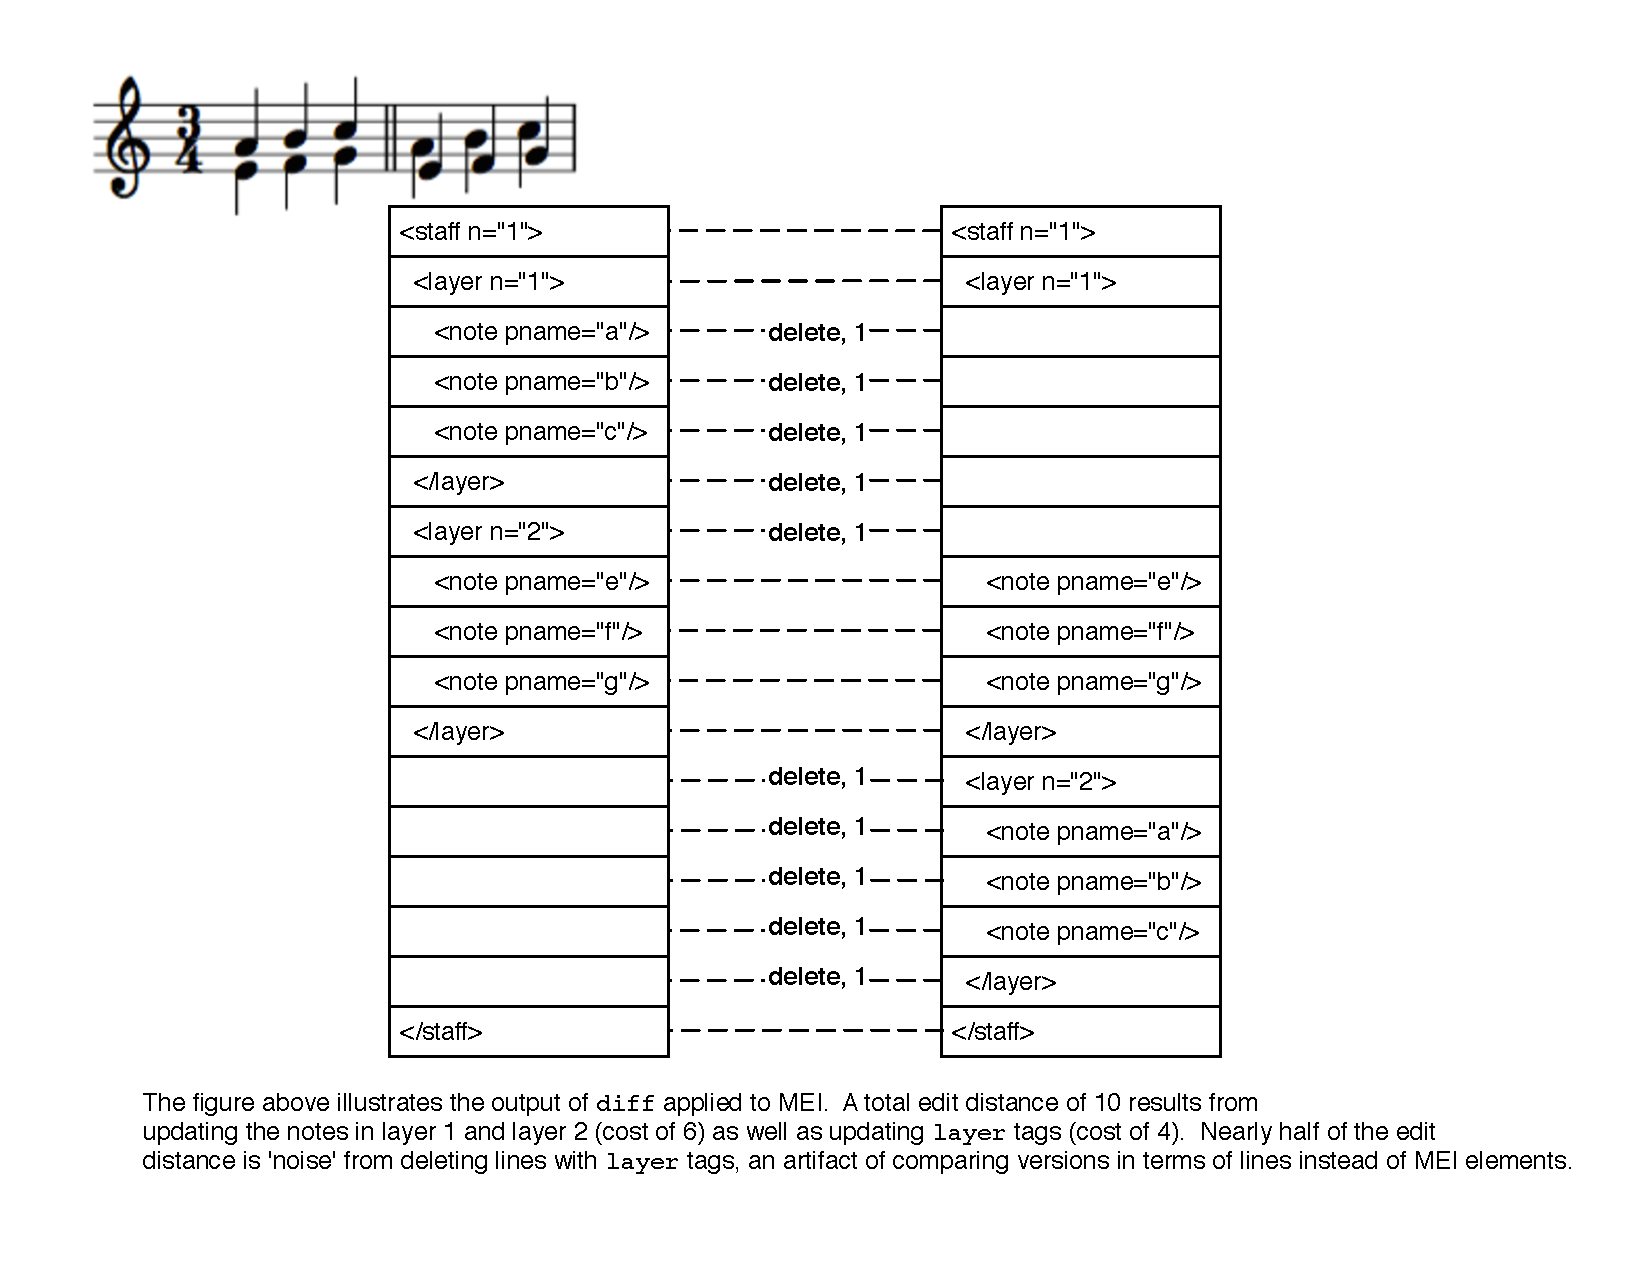
\includegraphics[width=\textwidth]{figure1.pdf}
\caption{The figure above illustrates the output of \texttt{diff} applied to MEI. A total edit distance of 10 results from updating the notes in layers 1 and 2 (cost of 6), as well as updating \texttt{layer} tags (cost of 4). "Noise" from layer tag deletion -- an artifact of line-based comparison rather than MEI element-based comparison -- makes up nearly half of the edit distance. }
\label{fig:example}
\end{figure*}

\begin{figure*}[!htb]
\centering
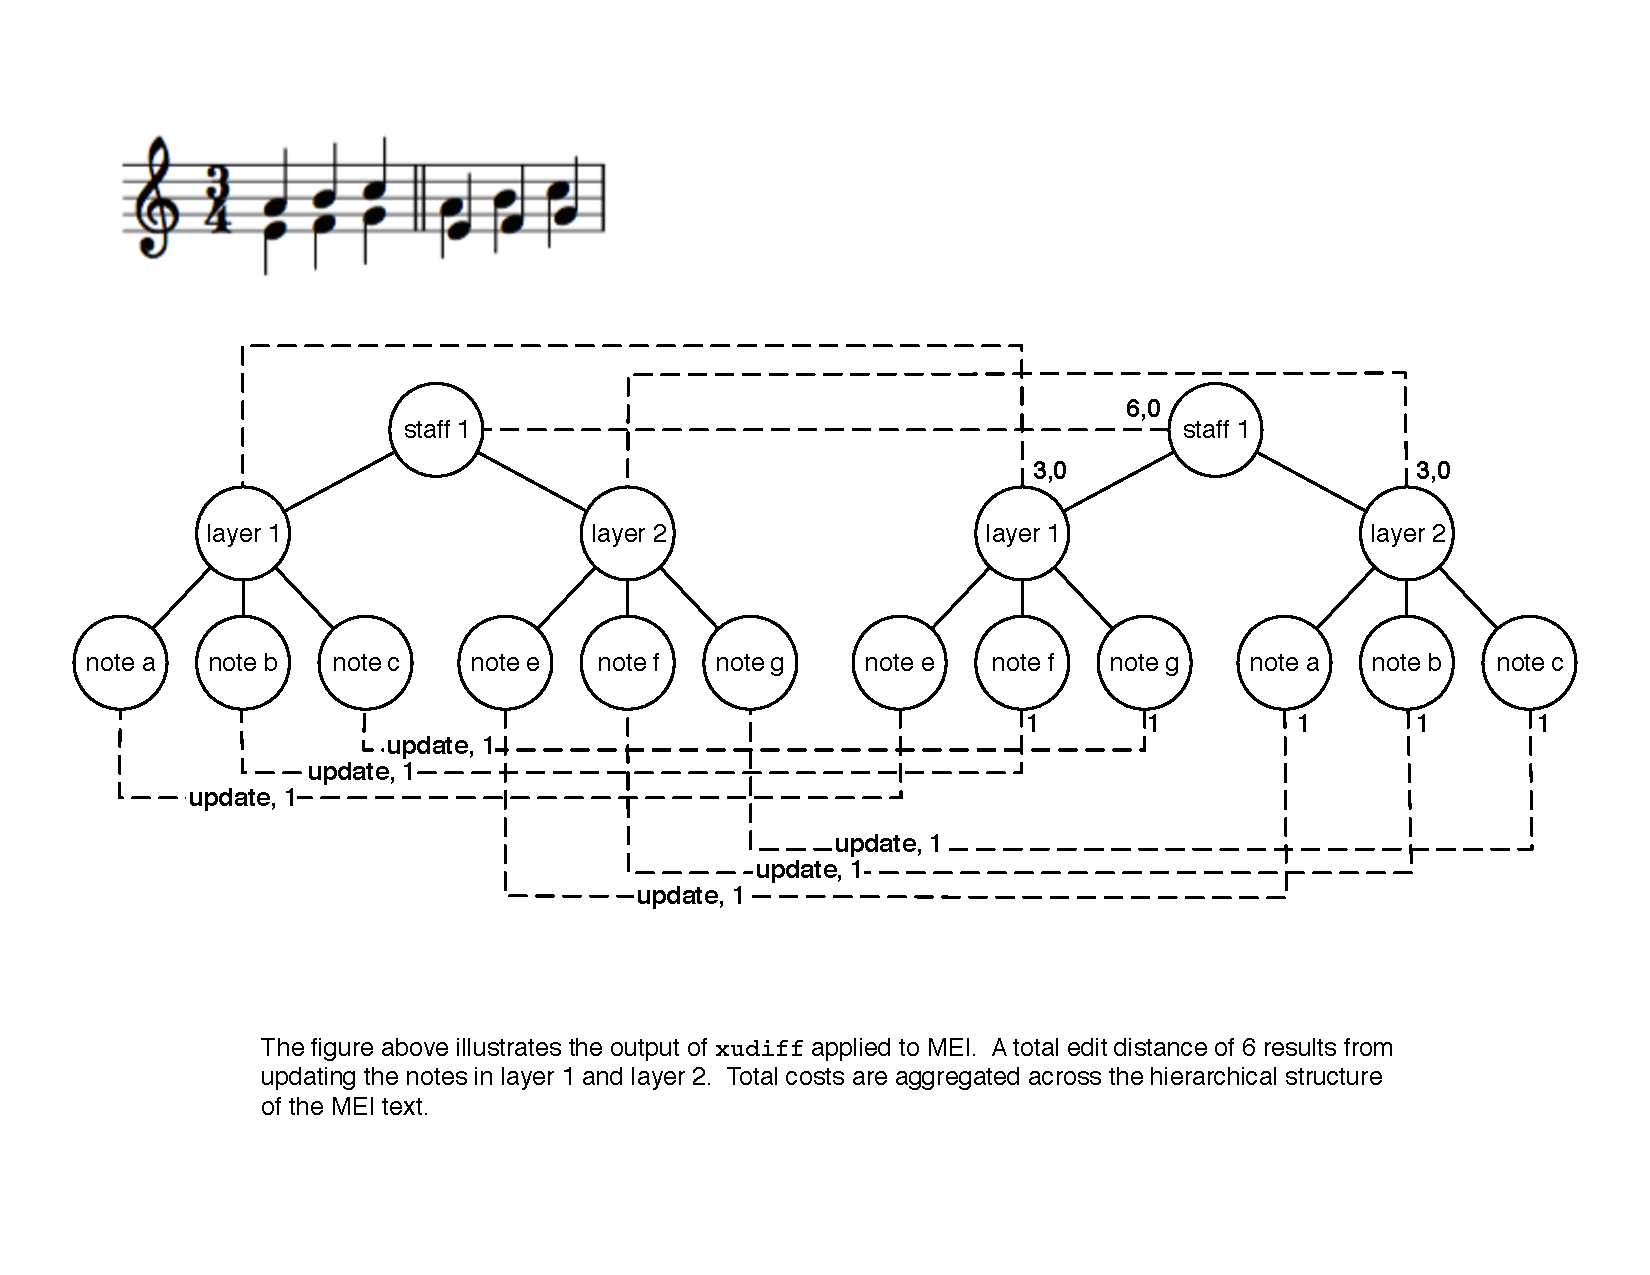
\includegraphics[width=\textwidth]{figure2.pdf}
\caption{The figure above illustrates the output of \texttt{xudiff} applied to MEI. A total edit distance of 6 results from updating the notes in layers 1 and 2. \texttt{xudiff} aggregates total costs across MEI's hierarchical structure: 3 for each layer and 6 for the staff.}
\label{fig:example}
\end{figure*}

% Jeffrey, please see p. 121 of my thesis for citations
%  What is the related work for this approach in general and
%  specifically to music composition?


\section{Conclusions}
The recently emerged potentials of online collaborative music applications illustrate several ways a robust hierarchic diff algorithm for music can enable newly collaborative musicology, composition, and music education through document utilities\cite{wust2001architectural,Martin:2015pb,McCulloch:2015pd,Flat:aa,Baca:2015xr}. Yet the commercial presentation of widely used digital engraving tools still conflates the act of sharing with act of collaboration, although these remain distinct from one another -- as a recent advertisement for the Sibelius engraving program exhorts, ``Collaborate more easily with others and distribute your compositions for the world to hear. Share scores through email, upload and publish them as sheet music on ScoreExchange.com, and even share your composition as a video or audio file on YouTube, Facebook, and SoundCloud'' \cite{Avid:to}. While file exchange between musical authors remains a crucial part of musical creativity and collaboration beyond notation, it is time for engraving software to embrace the potentials of genuinely collaborative music document editing interfaces. 

To explore these potential applications, the authors will implement the described algorithm as part of the nCoda project, an open-source interface for collaborative MEI document editing. The algorithm's integration into this project also invites the design of novel graphical user interfaces and diff representation that may take into account the user's music literacy.

%
\begin{acknowledgments}
Research conducted toward the nCoda project has been supported by Colorado College's SEGway faculty support grant.
\end{acknowledgments} 

%%%%%%%%%%%%%%%%%%%%%%%%%%%%%%%%%%%%%%%%%%%%%%%%%%%%%%%%%%%%%%%%%%%%%%%%%%%%%
%bibliography here
\balance
\clearpage
\bibliography{tenor2017diffs}

\end{document}
